%!TEX root = ../template.tex
%%%%%%%%%%%%%%%%%%%%%%%%%%%%%%%%%%%%%%%%%%%%%%%%%%%%%%%%%%%%%%%%%%%%
%% chapter3.tex
%% NOVA thesis document file
%%
%% Chapter with a short latex tutorial and examples
%%%%%%%%%%%%%%%%%%%%%%%%%%%%%%%%%%%%%%%%%%%%%%%%%%%%%%%%%%%%%%%%%%%%

\typeout{NT FILE chapter3.tex}%

\chapter{State Of The Art}
\label{cha:State_Of_The_Art}

The state of the art outlines the most relevant and advanced work currently available in the area covered by this work. 
It provides an overview of existing research, tools, and methodologies, helping to frame the context in which this work is situated. 
By reviewing what has already been accomplished, this section highlights ongoing challenges and uncovers the gaps that this work 
aims to address.

\section{Certified Compilers}
\label{sec:Certified_Compilers}

A compiler is a software system that translates a program written in a source programming language into an equivalent representation 
in a target language, typically a lower-level language such as assembly or machine code. The goal of a compiler is not only to preserve 
the semantics of the original program but also to generate efficient and executable code for the target platform.~\cite{AhoSU86}

A central challenge in compiler technology is: How can we trust compilers?. As discussed previously, compilers are 
inherently complex systems, particularly optimizing compilers, which perform intricate symbolic transformations. 
Despite rigorous testing practices, compilers can still introduce subtle bugs during these transformations. Such bugs are often 
extremely difficult to detect and diagnose~\cite{Leroy09-back-end}, as they may lead to unexpected program crashes, 
incorrect behaviour, or silent miscomputations in the generated code, even when the original source code remains syntactically and 
semantically valid.

This raises serious concerns in the context of safety-critical or high-assurance software, where traditional validation 
through testing alone is insufficient. In such domains, testing must be complemented or in some cases replaced by formal methods, 
such as model checking, static analysis, and deductive program verification~\cite{Leroy09-back-end}.

This is precisely where certified compilers become essential. A certified compiler is accompanied by a machine-checked formal proof 
that guarantees semantic preservation during the transformation from source to target code. It preserves the semantics of the source 
program during its transformation into target code. This approach offers strong assurances about the absence of certain classes of 
errors, such as compilation bugs, compilation inaccuracies, or unsafe optimizations~\cite{Leroy09}. Unlike traditional compilers, 
whose correctness is typically established through empirical testing or informal reasoning, certified compilers provide mathematical 
guarantees of correctness, making them valuable in the development of high-assurance and safety-critical software.

\subsection{CompCert}
\label{sec:CompCert}

The development of a realistic and verified compiler began with CompCert. Here, verified denotes a compiler accompanied by
a machine-checked proof that the generated code behaves exactly as prescribed by the semantics of the source program.
Realistic refers to a compiler that can be effectively employed in the production of critical software systems~\cite{Leroy09-back-end}.

CompCert adopts a multi-pass compilation architecture, where each pass translates an intermediate representation into a lower-level 
form, gradually transforming the high-level C source code into target assembly code. These intermediate languages are Clight, Cminor, 
RTL, LTL, and others are themselves formally defined within Coq. CompCert's core is implemented in Gallina, the functional programming 
language of Coq, which is based on the Calculus of Inductive Constructions, a powerful higher-order logic and typed $\lambda$-calculus. 
This implementation enables formal reasoning and machine-checked proofs of correctness for each compilation phase~\cite{MonniauxB22}.

Although CompCert is developed in Coq, it is not executed within the proof assistant. Instead, the verified Gallina code is extracted 
to \ocaml, where it is combined with a small portion of handwritten \ocaml code to produce an efficient and executable 
compiler~\cite{MonniauxB22}.

Since the compiler must generate a large subset of the C language, the code needs to be efficient enough and compact enough to fit the 
requirements of critical embedded systems. This implies a multi-pass compiler that features good register allocation and some basic 
optimizations~\cite{Leroy09-back-end}.


\subsection{CakeML}
\label{sec:CakeML}

\section{Pipeline}
\label{sec:Pipeline}

Some parts of the verification pipeline have already been implemented or require only minor adjustments to meet their 
objectives. \cameleer provides translation of \ocaml code annotated with \gospel specifications into \whyml :

\begin{figure}[H]
    \centering
    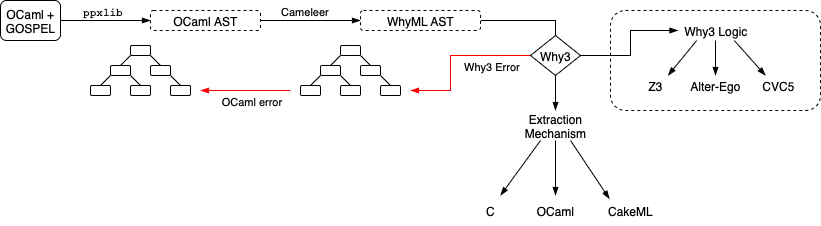
\includegraphics[width=\linewidth]{images/Cameleer.png}
    \caption{\ocaml to \whyml pipeline with \cameleer}
    \label{fig:Cameleer_pipeline}
\end{figure}

The extraction process does not require the correctness of the code to be proven. This may lead to potentially incorrect \ocaml 
programs to be extracted to \cml. Additionally, it is not designed to prevent users from extracting code even if the \gospel 
specifications can not guarantee correctness.

%%Processo de extracao nao esta ligado ao facto de um exemplo ja ter sido provado ou nao, pode potencialmente 
%%levar a gerar codigo cakeml nao correto

By modifying the extraction process in \whythree to check if the proof has been discharged we can provide better correctness 
guarantees because the generated \cml code will comply to the specification. Due to differences in syntax and features that 
have no direct equivalents in \cml, we must also include some kind of error message for failures in extraction, for instance 
the lack of support for while and for loops.

The goal of this work is to expand the currently available pipeline of translating code from \ocaml with \gospel specifications 
into \whyml, where it can be verified using the various automated provers available in Why3. One of our goals is to achieve 
a more robust extraction mechanism with the ideas as previously discussed. Moreover, we ought to provide a new tool that 
translates compilable \cml programs into \ocaml equivalents that can be specified afterwards with \gospel so that one may prove 
their correctness in \cameleer.

\begin{figure}[H]
    \centering
    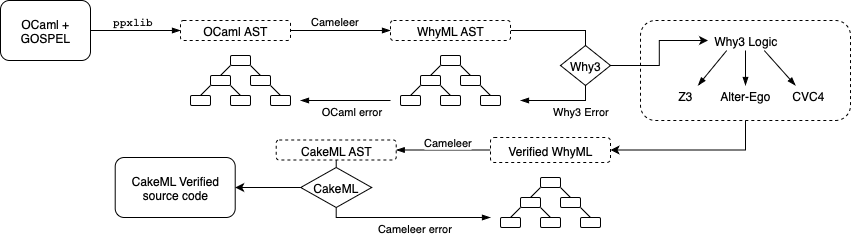
\includegraphics[width=\linewidth]{images/Goal_Pipeline.png}
    \caption{Goal pipeline}
\end{figure}



%%existe extracao cameleer para whyml, de whyml para cakeml, whyml para ocaml64